\subsection{iOS}
	Eine Applikation unter iOS kommuniziert wie unter Android ebenso (Kapitel:
	\ref{sec:app-android}) nicht direkt mit der Hardware sondern mit den dazwischen
	liegenden nativ gegebenen Schnittstellen, welche wie ein Schichtensystem
	angesehen werden können. Dabei nimmt die Komplexität, ebenso wie
	Nutzungsmöglichkeiten pro hinzu kommender Schicht zu. Durch diese vorgegebene
	Art der Hardwarenutzung wird ein immer gleich bleibender Standard und eine
	gewisse Einheitlichkeit garantiert.
	\begin{figure}[h]
		\centering
		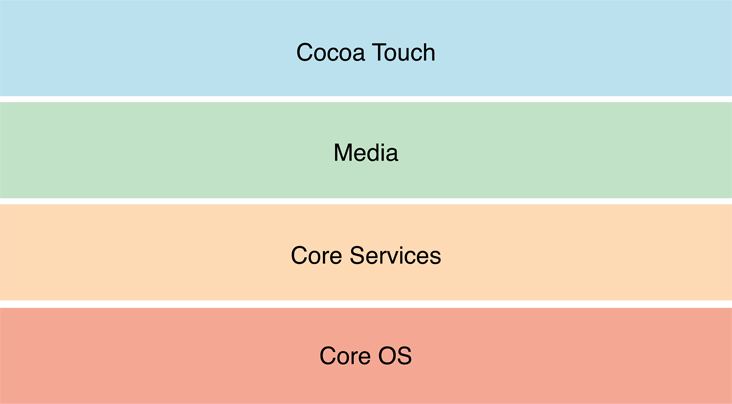
\includegraphics[width=0.5\linewidth]{ios/media/ios-layers.png}
		\caption{Ebenen der iOS Applikationsstruktur}
		%\cite{MobileOsStat}}
		\label{fig:marcetshare}
	\end{figure}
	
	\subsubsection{Technologien zur App-Entwicklung}
		IOS bietet eine Fülle an Bibliotheken an, welche von der tiefen und
		hardwarenahen Programmierung abstrahieren. Dies ermöglicht mit weniger
		Programmierlogik mehr zu erreichen und eventuell komplexe Aufgaben, wie
		Speicherallokation oder Multithreading an tiefere Schichten abzugeben.
		%TODO: cite
		% https://developer.apple.com/library/ios/documentation/Miscellaneous/Conceptual/iPhoneOSTechOverview/Introduction/Introduction.html#//apple_ref/doc/uid/TP40007898-CH1-SW1
		Apple empfiehlt eine Arbeitsweise auf möglichst abstrahierter Ebene.
		Nachfolgend wird auf einzelne Bestandteile dieser Schichtenarchitektur
		eingegangen. Es gilt hier anzumerken, dass nur wenige genannt werden, da die
		Nennung und Erläuterung aller den Rahmen dieser Arbeit überlaufen würde.
		\paragraph{Cocoa Touch Layer}
			Das \textsl{Cocoa Touch Framework} enthält Bibliotheken welche unter anderem
			für das Erscheinungsbild einer App verantwortlich sind. Zusätzlich werden
			Möglichkeiten für Multitasking, Push-Benachrichtigungen, Gestenerkennung und
			viele weitere Schnittstellen auf höherer Programmierebene, wie beispielsweise
			das Twitter-Framework geboten.
		\paragraph{Media Layer}
			In der \textsl{Medien Ebene} werden Bibliotheken, für
			Audio-, Video- und Bildbearbeitung gespeichert. Außerdem existiert hier die
			Schnittstelle für Apple's \textsl{AirPlay} - einem Video und Audiostreaming
			Dienst für Apple TV und Drittanbieter Lautsprecher beziehungsweise Empfänger.
		\paragraph{Core Services Layer}
			Auf der dritten Schicht - den Kerndienstleistungen des Systems werden
			Schnittstellen für Peer-to-Peer und andere Netzwerktechnologien angeboten.
			Weiterhin ist es möglicht auf den iCloud Dienst, dem unter Kapitel
			\ref{sec:filesecurity} dokumentierten sicherheitsessentiellen \textsl{Data
			Protection}, sowie die SQLite Unterstützung zurückzugreifen.
		\paragraph{Core OS Layer}
			Die unterste der vier Schichten liegt am hardwarenahesten und hält somit
			Möglichkeiten auf den Zugriff dieser vor. Dazu zählen das \textsl{Accelerate
			Framework} - unter anderem für Bildbearbeitung und lineare Algebra sowie das
			\textsl{Core Bluetooth Framework} - speziell für die Kommunikation mit
			Bluetooth LE\footnote{LE: Low-Energy} Geräten. Außerdem wird ab iOS 7
			die Unterstützung für native 64-Bit Apps angeboten. Als ein der wichtigsten
			Komponenten soll zuletzt das \textsl{Security Framework} erwähnt werden.
			Dieses bietet Schnittstellen für das Management von Zertifikaten, Richtlinien
			und privaten, sowie öffentlichen Schlüsseln. Außerdem wird das Erstellen von
			Zufallszahlen durch den in Kapitel \ref{sec:crypto-engine}
			vorgestellten \textsl{Random Number Generator} unterstützt, sowie die
			Verwendung von symmetrischer Verschlüsselung durch die unter Kapitel
			\ref{sec:3cc} vorgestellte Bibliothek \textsl{Common Crypto Library}.
